\documentclass[border=4pt]{standalone}
% Shared TikZ preamble for book diagrams
% Usage: % Shared TikZ preamble for book diagrams
% Usage: % Shared TikZ preamble for book diagrams
% Usage: \input{../preamble.tex} after \documentclass

\usepackage{tikz}
\usepackage{amsmath,amssymb}

\usetikzlibrary{arrows.meta, calc, positioning, decorations.pathreplacing}

% --- Color palette ---
% Consistent across all diagrams in the book
\definecolor{basis1}{RGB}{31,119,180}    % blue: encoders, structure
\definecolor{msg}{RGB}{44,160,44}        % green: positives
\definecolor{aux}{RGB}{127,127,127}      % gray: alternatives, auxiliary
\definecolor{highlight}{RGB}{255,127,14} % orange: highlights
\definecolor{lightfill}{RGB}{230,240,255}% light blue: shaded regions

% --- Reusable styles ---
\tikzset{
  encoder/.style={draw=basis1!60, fill=lightfill, rounded corners=3pt,
    minimum width=1.0cm, minimum height=0.8cm},
  flow/.style={-{Stealth[length=5pt,width=4pt]}, line width=0.8pt},
  annotation/.style={font=\footnotesize, text=aux!80!black},
}
 after \documentclass

\usepackage{tikz}
\usepackage{amsmath,amssymb}

\usetikzlibrary{arrows.meta, calc, positioning, decorations.pathreplacing}

% --- Color palette ---
% Consistent across all diagrams in the book
\definecolor{basis1}{RGB}{31,119,180}    % blue: encoders, structure
\definecolor{msg}{RGB}{44,160,44}        % green: positives
\definecolor{aux}{RGB}{127,127,127}      % gray: alternatives, auxiliary
\definecolor{highlight}{RGB}{255,127,14} % orange: highlights
\definecolor{lightfill}{RGB}{230,240,255}% light blue: shaded regions

% --- Reusable styles ---
\tikzset{
  encoder/.style={draw=basis1!60, fill=lightfill, rounded corners=3pt,
    minimum width=1.0cm, minimum height=0.8cm},
  flow/.style={-{Stealth[length=5pt,width=4pt]}, line width=0.8pt},
  annotation/.style={font=\footnotesize, text=aux!80!black},
}
 after \documentclass

\usepackage{tikz}
\usepackage{amsmath,amssymb}

\usetikzlibrary{arrows.meta, calc, positioning, decorations.pathreplacing}

% --- Color palette ---
% Consistent across all diagrams in the book
\definecolor{basis1}{RGB}{31,119,180}    % blue: encoders, structure
\definecolor{msg}{RGB}{44,160,44}        % green: positives
\definecolor{aux}{RGB}{127,127,127}      % gray: alternatives, auxiliary
\definecolor{highlight}{RGB}{255,127,14} % orange: highlights
\definecolor{lightfill}{RGB}{230,240,255}% light blue: shaded regions

% --- Reusable styles ---
\tikzset{
  encoder/.style={draw=basis1!60, fill=lightfill, rounded corners=3pt,
    minimum width=1.0cm, minimum height=0.8cm},
  flow/.style={-{Stealth[length=5pt,width=4pt]}, line width=0.8pt},
  annotation/.style={font=\footnotesize, text=aux!80!black},
}

\begin{document}
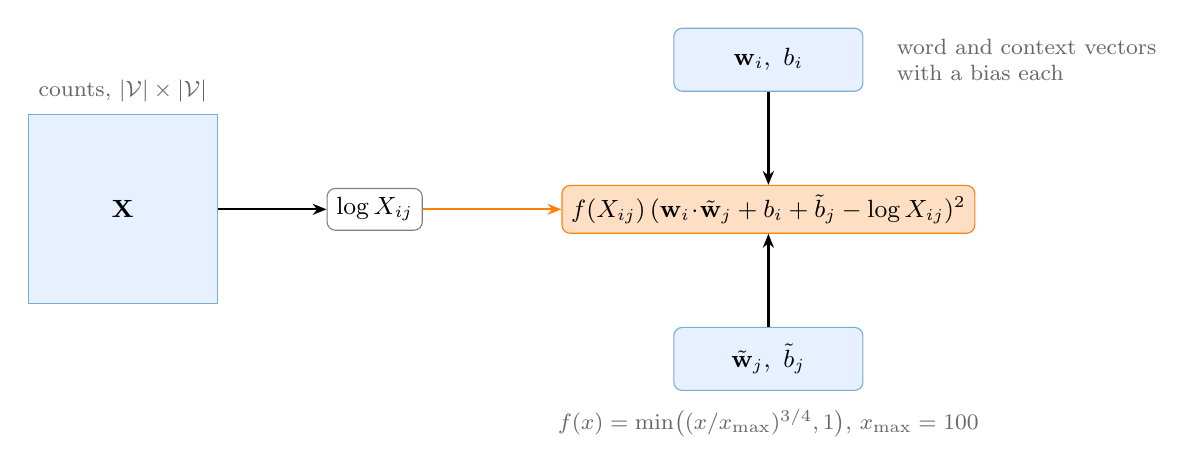
\begin{tikzpicture}[font=\small]
  \node[draw=basis1!60, fill=lightfill, minimum width=2.4cm, minimum height=2.4cm] (X) at (0,0) {$\mathbf{X}$};
  \node[annotation, above=1pt of X] {counts, $|\mathcal{V}|\times|\mathcal{V}|$};
  \node[draw=aux, rounded corners=3pt] (L) at (3.2,0) {$\log X_{ij}$};
  \draw[flow] (X) -- (L);
  \node[draw=highlight, fill=highlight!25, rounded corners=3pt] (J) at (8.2,0) {$f(X_{ij})\,(\mathbf{w}_i\!\cdot\!\tilde{\mathbf{w}}_j+b_i+\tilde b_j-\log X_{ij})^2$};
  \draw[flow, highlight] (L) -- (J);
  \node[encoder, minimum width=2.4cm] (W) at (8.2,1.9) {$\mathbf{w}_i,\ b_i$};
  \node[encoder, minimum width=2.4cm] (Wt) at (8.2,-1.9) {$\tilde{\mathbf{w}}_j,\ \tilde b_j$};
  \draw[flow] (W) -- (J);
  \draw[flow] (Wt) -- (J);
  \node[annotation, align=center, below=3pt of Wt] {$f(x)=\min\!\big((x/x_{\max})^{3/4},1\big)$, $x_{\max}=100$};
  \node[annotation, align=left, anchor=west] at ([xshift=0.3cm]W.east) {word and context vectors\\with a bias each};
\end{tikzpicture}
\end{document}
